% ============================================================================
% ex1.tex
% ============================================================================
% Exercício individual da lista.
% Este arquivo deve conter apenas o conteúdo do exercício e, quando desejado,
% sua resolução. Não deve carregar pacotes nem redefinir configurações globais.
%
% Interface adotada neste exemplo:
% - ambiente `exercicio` com identificador textual livre;
% - ambiente `resolucao` para a solução;
% - subseções internas apenas para organizar a exposição.
% ============================================================================

\begin{exercicio}[Problem 1 --- SHG with Gaussian Beams]
Consider the problem of Second Harmonic Generation (SHG) with Gaussian beams. We have discussed how in this case the effective nonlinear coefficient carries an overlap integral that depends on the matching between the interacting fields.

\begin{enumerate}[a)]
\item Show with a numerical simulation that the Boyd-Kleinman criterion arises from optimizing this overlap integral.
\item Discuss how the phase mismatch is affected when Gaussian beams are used instead of plane waves.
\end{enumerate}
\end{exercicio}

\begin{resolucao}[Solution]

\subsection*{(a) Numerical Optimization of the Overlap Integral}

    \paragraph*{Theoretical Framework}
        The analytical treatment of nonlinear interactions with focused Gaussian beams is given in \textbf{Section 2.10 of \authorlinkcite{Boyd}} (4th edition, \textit{Nonlinear Optical Interactions with Focused Gaussian Beams}, pp.~109--116). In particular, the derivation used here is based on \textbf{Section 2.10.3} (\textit{Harmonic Generation Using Focused Gaussian Beams}, pp.~112--116), where Boyd writes the driven paraxial equation for the generated harmonic field in Eq.~(2.10.7), represents the fundamental Gaussian beam in Eq.~(2.10.8), introduces the harmonic-field trial solution in Eq.~(2.10.9), and obtains the longitudinal generation integral in Eq.~(2.10.11b). The optimum focusing result quoted by Boyd and Kleinman is stated explicitly after Fig.~2.10.4 and summarized in Eq.~(2.10.14), where Boyd reports the optimum values $L/b=2.84$, $\Delta k=3.2/L$, and the numerical coefficient $K=1.068$ for the original Gaussian-units normalization.
    
        The propagation properties of a Gaussian beam are taken from \textbf{Section 3.1 of \authorlinkcite{Saleh}} (\textit{The Gaussian Beam}, pp.~80--88). In that section, Saleh and Teich write the Gaussian beam complex amplitude in Eq.~(3.1-7), the beam radius in Eq.~(3.1-8), the radius of curvature in Eq.~(3.1-9), the Gouy phase function in Eq.~(3.1-10), and the Rayleigh range in Eq.~(3.1-11). Their Eq.~(3.1-22) identifies the confocal parameter, or depth of focus, as twice the Rayleigh range. In the notation used below, I write this quantity as
        \begin{equation}
            b = 2z_R = \frac{2\pi n_1 w_0^2}{\lambda_1},
            \label{eq:confocal_parameter_saleh}
        \end{equation}
        which is the same physical parameter denoted by Boyd in Eq.~(2.10.5c), except that Boyd writes it as $b=2\pi w_0^2/\lambda$ when the wavelength $\lambda$ is already the wavelength inside the medium.

        Thus, the calculation below combines two ingredients from the references:
        \begin{itemize}
            \item the Gaussian-beam geometry and Gouy phase from Saleh and Teich, Sec.~3.1;
            \item the nonlinear overlap integral for harmonic generation with focused beams from Boyd, Sec.~2.10.3.
        \end{itemize}

    \paragraph*{From Boyd's Longitudinal Integral to the Boyd-Kleinman Factor}
        Boyd's Eq.~(2.10.11b) gives the longitudinal integral controlling the generated $q$-th harmonic amplitude:
        \begin{equation}
            J_q(\Delta k,z_0,z)
            =
            \int_{z_0}^{z}
            \frac{
            e^{i\Delta k z'}
            }{
            \left(1+2iz'/b\right)^{q-1}
            }
            dz',
            \label{eq:boyd_Jq_dimensional}
        \end{equation}
        where $\Delta k=qk_1-k_q$. For SHG, $q=2$, so this reduces to
        \begin{equation}
            J_2(\Delta k,z_0,z)
            =
            \int_{z_0}^{z}
            \frac{
            e^{i\Delta k z'}
            }{
            1+2iz'/b
            }
            dz'.
            \label{eq:J2_dimensional}
        \end{equation}
        The problem statement assumes the standard Boyd-Kleinman geometry: the waist of the fundamental Gaussian beam is placed at the center of a nonlinear crystal of length $L$. Therefore, the input and output faces are located at
        \begin{equation}
            z_0=-\frac{L}{2},
            \qquad
            z=+\frac{L}{2}.
        \end{equation}
        Introducing the dimensionless coordinate
        \begin{equation}
            \tau = \frac{2z'}{b},
            \qquad
            dz'=\frac{b}{2}\,d\tau,
        \end{equation}
        the limits become
        \begin{equation}
            z'=-\frac{L}{2}\Rightarrow \tau=-\frac{L}{b}=-\xi,
            \qquad
            z'=+\frac{L}{2}\Rightarrow \tau=+\frac{L}{b}=+\xi,
        \end{equation}
        where
        \begin{equation}
            \xi=\frac{L}{b}.
            \label{eq:xi_definition}
        \end{equation}
        Similarly, the phase factor becomes
        \begin{equation}
            \Delta k z'
            =
            \Delta k \frac{b\tau}{2}
            =
            \sigma \tau,
            \qquad
            \sigma=\frac{1}{2}b\Delta k.
            \label{eq:sigma_definition}
        \end{equation}
        Thus, apart from the dimensional prefactor $b/2$, the relevant dimensionless overlap amplitude is
        \begin{equation}
            \mathcal I(\sigma,\xi)
            =
            \int_{-\xi}^{+\xi}
            \frac{
            e^{i\sigma\tau}
            }{
            1+i\tau
            }
            d\tau.
            \label{eq:full_dimensionless_overlap}
        \end{equation}
        This equation is the dimensionless version of Boyd's Eq.~(2.10.11b) specialized to second-harmonic generation and to a crystal centered at the Gaussian waist.

    \paragraph*{Where the Symmetry Factor Enters}
        The factor of two associated with the symmetry of the problem enters when the full integral in Eq.~\eqref{eq:full_dimensionless_overlap}, over $[-\xi,+\xi]$, is rewritten as an integral over $[0,\xi]$.

        To see this explicitly, define
        \begin{equation}
            f(\tau)
            =
            \frac{
            e^{i\sigma\tau}
            }{
            1+i\tau
            }.
        \end{equation}
        Then
        \begin{equation}
            \mathcal I(\sigma,\xi)
            =
            \int_0^\xi
            \left[
            f(\tau)+f(-\tau)
            \right]d\tau.
        \end{equation}
        Now,
        \begin{align}
            f(\tau)
            &=
            \frac{e^{i\sigma\tau}}{1+i\tau}
            =
            \frac{
            \left[\cos(\sigma\tau)+i\sin(\sigma\tau)\right](1-i\tau)
            }{
            1+\tau^2
            }
            \nonumber\\
            &=
            \frac{
            \cos(\sigma\tau)+\tau\sin(\sigma\tau)
            }{
            1+\tau^2
            }
            +
            i
            \frac{
            \sin(\sigma\tau)-\tau\cos(\sigma\tau)
            }{
            1+\tau^2
            }.
        \end{align}
        The real part is an even function of $\tau$, while the imaginary part is an odd function of $\tau$. Therefore, the imaginary contribution cancels over the symmetric interval, and one obtains
        \begin{equation}
            \mathcal I(\sigma,\xi)
            =
            2
            \int_0^\xi
            \frac{
            \cos(\sigma\tau)+\tau\sin(\sigma\tau)
            }{
            1+\tau^2
            }
            d\tau.
            \label{eq:symmetric_amplitude_integral}
        \end{equation}

        This is the point at which care is required. The factor $2$ in Eq.~\eqref{eq:symmetric_amplitude_integral} is indeed a symmetry factor, but it belongs to the \emph{amplitude integral} $\mathcal I$. The dimensionless Boyd-Kleinman efficiency factor is proportional to the squared modulus of the full overlap amplitude with the standard normalization
        \begin{equation}
            h(\sigma,\xi)
            =
            \frac{1}{4\xi}
            \left|
            \mathcal I(\sigma,\xi)
            \right|^2.
            \label{eq:h_full_integral_definition}
        \end{equation}
        Substituting Eq.~\eqref{eq:symmetric_amplitude_integral} into Eq.~\eqref{eq:h_full_integral_definition}, the factor $2$ from the amplitude is squared and cancels the factor $4$ in the denominator:
        \begin{align}
            h(\sigma,\xi)
            &=
            \frac{1}{4\xi}
            \left|
            2
            \int_0^\xi
            \frac{
            \cos(\sigma\tau)+\tau\sin(\sigma\tau)
            }{
            1+\tau^2
            }
            d\tau
            \right|^2
            \nonumber\\
            &=
            \frac{1}{\xi}
            \left[
            \int_0^\xi
            \frac{
            \cos(\sigma\tau)+\tau\sin(\sigma\tau)
            }{
            1+\tau^2
            }
            d\tau
            \right]^2.
            \label{eq:boyd_kleinman}
        \end{align}
        Therefore, in the half-interval form used for the numerical calculation, the correct expression is
        \begin{equation}
            \boxed{
            h(\sigma, \xi)
            =
            \frac{1}{\xi}
            \left[
            \int_{0}^{\xi}
            \frac{
            \cos(\sigma \tau)+\tau \sin(\sigma \tau)
            }{
            1+\tau^2
            }
            d\tau
            \right]^2
            }.
            \label{eq:boyd_kleinman_corrected}
        \end{equation}

        This explains why the prefactor must be $1/\xi$, not $2/\xi$, once the integral has already been reduced to the interval $[0,\xi]$. If one used $2/\xi$ in Eq.~\eqref{eq:boyd_kleinman_corrected}, the location of the maximum in the $(\sigma,\xi)$ plane would remain essentially the same, because multiplying the objective function by a constant does not move its maximum. However, the numerical value of the maximum would be doubled. That would give a peak close to $2.14$ instead of the Boyd-Kleinman value $1.068$ quoted by Boyd after Eq.~(2.10.14). Thus, the normalization with $1/\xi$ is the one consistent with the standard Boyd-Kleinman efficiency factor.

    \paragraph*{Numerical Optimization}
        To find the conditions for maximum conversion efficiency, Eq.~\eqref{eq:boyd_kleinman_corrected} was evaluated over a bidimensional grid of the parameters $\xi$ and $\sigma$. The complete algorithm execution and visualization can be found in Appendix~\ref{app:boyd-kleinman-code}.

        The numerical maximization yields the classical Boyd-Kleinman optimization criterion:
        \begin{equation}
            \xi_{\mathrm{opt}}
            \approx 2.84
            \qquad
            \text{and}
            \qquad
            \sigma_{\mathrm{opt}}
            \approx 0.57.
            \label{eq:bk_optimum_sigma_xi}
        \end{equation}
        This is consistent with Boyd's statement in Sec.~2.10.3 that the highest SHG efficiency is obtained when the beam waist is placed at the center of the crystal, the ratio $L/b$ is equal to $2.84$, and the wavevector mismatch is set to
        \begin{equation}
            \Delta k_{\mathrm{opt}}
            =
            \frac{3.2}{L}.
            \label{eq:boyd_delta_k_optimum}
        \end{equation}
        Indeed, using the definitions $\xi=L/b$ and $\sigma=b\Delta k/2$, one obtains
        \begin{equation}
            \Delta k
            =
            \frac{2\sigma}{b}
            =
            \frac{2\sigma\xi}{L}.
        \end{equation}
        Substituting the numerical optimum from Eq.~\eqref{eq:bk_optimum_sigma_xi},
        \begin{equation}
            \Delta k_{\mathrm{opt}}
            =
            \frac{
            2(0.57)(2.84)
            }{
            L
            }
            \approx
            \frac{3.24}{L}
            \approx
            \frac{3.2}{L},
        \end{equation}
        in agreement with Boyd's quoted Boyd-Kleinman result.

        At this global maximum, the efficiency factor reaches
        \begin{equation}
            h(\sigma_{\mathrm{opt}},\xi_{\mathrm{opt}})
            \approx 1.068.
        \end{equation}
        This reproduces the numerical factor reported by Boyd in connection with Eq.~(2.10.14). In physical terms, the highest SHG efficiency occurs when the crystal length is roughly three times the beam's confocal parameter,
        \begin{equation}
            L \approx 2.84b,
        \end{equation}
        rather than in either of the two limiting regimes:
        \begin{itemize}
            \item very weak focusing, where the beam area remains large and the intensity is small;
            \item very tight focusing, where the intensity is high near the waist but the effective interaction length is shortened by diffraction and by the accumulated Gouy phase.
        \end{itemize}

        \begin{figure}[H]
            \centering
            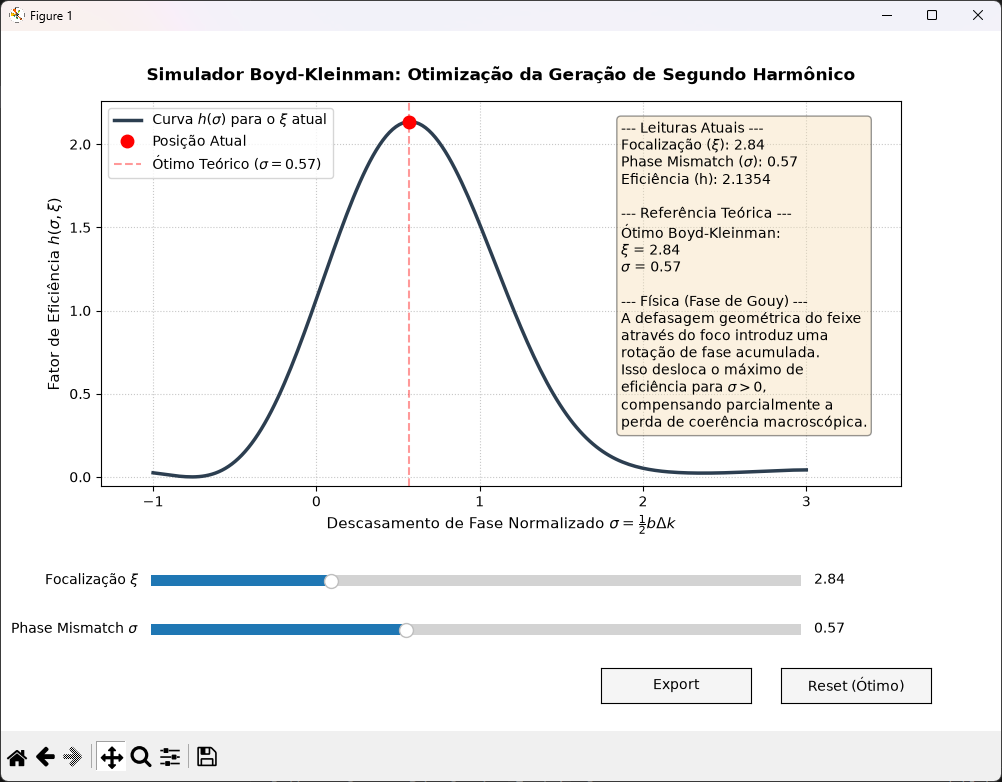
\includegraphics[width=0.75\columnwidth]{Interactive Boyd-Kleinman Simulator.png}
            \caption{Graphical User Interface (GUI) of the interactive script, developed to explore the influence of the Gouy phase shift on second-harmonic generation in real time.}
            \label{fig:simulator_gui}
        \end{figure}

        \begin{figure}[H]
            \centering
            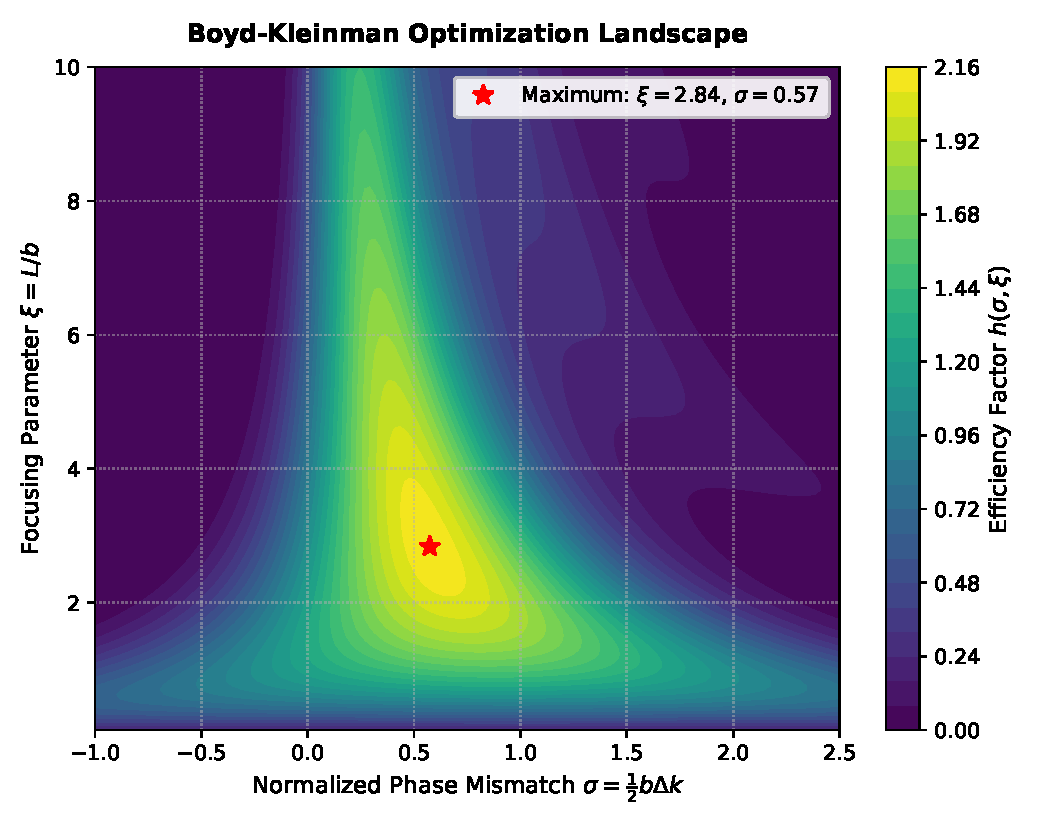
\includegraphics[width=\columnwidth]{boyd_kleinman_plot.pdf}
            \caption{Numerical evaluation of the Boyd-Kleinman factor $h(\sigma,\xi)$ as a function of the normalized phase mismatch $\sigma$ and focusing parameter $\xi$. The red star highlights the global optimum at $\xi \approx 2.84$ and $\sigma \approx 0.57$, where $h_{\max}\approx 1.068$.}
            \label{fig:boyd_kleinman}
        \end{figure}

\subsection*{(b) Phase Mismatch: Gaussian Beams vs. Plane Waves}

    The transition from the plane-wave regime to focused Gaussian beams introduces a fundamental shift in the phase-matching requirements. The reason is that a focused Gaussian beam is not merely a plane wave with finite transverse size: it has a longitudinally varying radius, a curved wavefront, and a Gouy phase. These features are described in Saleh and Teich, Sec.~3.1, especially Eqs.~(3.1-7)--(3.1-11) and the phase discussion around Eqs.~(3.1-23)--(3.1-24). In Boyd's nonlinear-optics treatment, the same physics enters through the denominator $(1+2iz/b)$ in Eq.~(2.10.11b), which modifies the longitudinal overlap integral relative to the plane-wave case.

    \paragraph*{Plane-Wave Limit}
        In the plane-wave limit, the beam is taken to have infinite transverse extent or, equivalently, a confocal parameter much larger than the nonlinear crystal length. In Boyd's notation this corresponds to the limit in which the denominator in Eq.~(2.10.11b) is approximately constant over the crystal. Boyd explicitly states this reduction in Eq.~(2.10.12a), obtaining
        \begin{equation}
            J_q(\Delta k,z_0,z)
            =
            \int_{z_0}^{z}
            e^{i\Delta k z'}dz'
            =
            \frac{
            e^{i\Delta k z}-e^{i\Delta k z_0}
            }{
            i\Delta k
            }.
            \label{eq:plane_wave_overlap}
        \end{equation}
        For an interaction length $L=z-z_0$, Boyd's Eq.~(2.10.12b) gives
        \begin{equation}
            |J_q|^2
            =
            L^2
            \operatorname{sinc}^2
            \left(
            \frac{\Delta k L}{2}
            \right).
            \label{eq:sinc_plane_wave}
        \end{equation}
        This is the usual plane-wave phase-matching factor. It reaches its maximum at
        \begin{equation}
            \Delta k=0.
        \end{equation}
        The same plane-wave SHG phase mismatch is defined in Boyd's Eq.~(2.7.12),
        \begin{equation}
            \Delta k = 2k_1-k_2,
        \end{equation}
        after the coupled-amplitude equation for the second-harmonic field in Eq.~(2.7.11). Thus, for plane waves, the mathematical and physical condition for maximum coherent buildup is simply perfect material phase matching.

    \paragraph*{The Role of the Gouy Phase Shift}
        For focused Gaussian beams, this conclusion is modified. The numerical result in Eq.~\eqref{eq:bk_optimum_sigma_xi} shows that the optimum mismatch shifts to
        \begin{equation}
            \sigma_{\mathrm{opt}}\approx 0.57,
        \end{equation}
        which implies a strictly nonzero material phase mismatch:
        \begin{equation}
            \Delta k_{\mathrm{opt}}
            =
            \frac{2\sigma_{\mathrm{opt}}}{b}
            >
            0.
        \end{equation}

        The physical origin of this shift is the Gouy phase. Saleh and Teich write the Gaussian beam phase in Eq.~(3.1-23) as containing, on axis, the term
        \begin{equation}
            \phi(0,z)=kz-\zeta_G(z),
        \end{equation}
        where, using the notation $\zeta_G$ to avoid confusion with Boyd's dimensionless coordinate,
        \begin{equation}
            \zeta_G(z)
            =
            \tan^{-1}
            \left(
            \frac{z}{z_R}
            \right).
        \end{equation}
        In Saleh and Teich's notation this function is denoted by $C(z)$ in Eq.~(3.1-10), with $z_0$ playing the role of the Rayleigh range. As the beam passes from $z=-\infty$ to $z=+\infty$, $\zeta_G(z)$ changes from $-\pi/2$ to $+\pi/2$, so the total Gouy phase change is $\pi$.

        In the nonlinear interaction, however, the source of the second-harmonic wave is not the fundamental field itself, but the nonlinear polarization
        \begin{equation}
            P_{\mathrm{NL}}(2\omega)\propto E_\omega^2.
        \end{equation}
        Therefore, if the fundamental field carries a Gouy phase contribution $\zeta_G(z)$, the nonlinear polarization driving SHG carries twice this contribution. This is exactly the qualitative point made by Boyd after Fig.~2.10.4: for $q$-th harmonic generation, the nonlinear polarization contains $A_1^q$ and therefore acquires a phase shift $q$ times larger than that of the incident fundamental field.

        If the material were perfectly phase matched in the plane-wave sense, $\Delta k=0$, the generated second-harmonic field and the nonlinear polarization would not remain optimally phased throughout the focal region. The geometric phase evolution associated with focusing would introduce a longitudinal phase slip. In a macroscopic crystal, contributions generated before and after the focus would then interfere less constructively, reducing the net SHG output.

        A positive wavevector mismatch compensates this geometric phase slip. In the notation used here, this means choosing
        \begin{equation}
            \Delta k>0,
        \end{equation}
        or, equivalently,
        \begin{equation}
            \sigma>0.
        \end{equation}
        This explains why the focused-beam optimum is not located at $\Delta k=0$, but instead at
        \begin{equation}
            \Delta k_{\mathrm{opt}}\approx \frac{3.2}{L}.
        \end{equation}
        The bulk material mismatch supplies a linear phase variation that compensates the nonlinear Gouy phase accumulated near the beam waist.

        Therefore, the focused Gaussian-beam problem differs from the plane-wave problem in two coupled ways:
        \begin{enumerate}
            \item the transverse confinement increases the intensity and therefore tends to increase the nonlinear conversion;
            \item the same confinement introduces diffraction and Gouy-phase effects, which modify the longitudinal phase-matching condition.
        \end{enumerate}
        The Boyd-Kleinman criterion is precisely the optimization of this trade-off. It selects the focusing parameter $\xi=L/b$ and the normalized mismatch $\sigma=b\Delta k/2$ that maximize the full Gaussian overlap integral, rather than the plane-wave $\operatorname{sinc}^2(\Delta kL/2)$ factor.

\end{resolucao}
